\documentclass[12pt]{article}  
%%Read the manual for other options. 

\pagestyle{empty} %%Eliminates page numbers
%%\input rmb_macros
%%Collect your favorite macros in a 
%%separate file

%\input amssym.def
%\input amssym
%\input mssymb
%%Defines additional symbols



\usepackage{graphics}
\usepackage{amsmath,amssymb,amsthm, multicol}
\usepackage[pdftex]{graphicx}
\usepackage{epsf}
%%Use to include pictures. 

%\newcommand{\comment}[1]{}
%\newcommand{\sobolev}[2]{W^{#1,#2}}
%\newcommand{\sobolev}[2]{L^#2_#1}
%%Some examples of macros or new commands.
\newcommand{\E}{\mathbb{E}}

\addtolength{\oddsidemargin}{-.75in}
\addtolength{\evensidemargin}{-.75in}
\addtolength{\textwidth}{1.5in}
\addtolength{\topmargin}{-1in}
\addtolength{\textheight}{2.25in}
%%Set margins, defaults are ok. 

\begin{document}
\begin{flushleft} 
%%Paragraphs will not be indented in this 
%%environment
\centerline{\LARGE{Quiz 8}} 
\vspace{5 mm}
{Form A}\hfill  
%%\hfill forces following text 
%%to right margin
{Name \rule {2 in}{0.01in}}\\
Math 130B, 5 PM
\\
%%gives a line of length 2in and 
%%thickness 0.01in
{Please justify all your answers}\hfill {May 25, 2022}
\\
{Please also write your full name on the back} 

\medskip
\end{flushleft}
\begin{enumerate}

	\item Suppose $X$ and $Y$ are independent random variables with the following moment generating functions.
	\[
		m_X(t) = e^{2t^2},\quad m_Y(t) = \frac{3}{3-t}.
	\]
	\begin{enumerate}
		\item What kinds of random variables are $X$ and $Y$? (There's a table on the back of the quiz).

		\vfill

		\item Find $\E[(X+Y)^2]$ (there are a couple of ways to do it).
	\end{enumerate}

	\vfill

	\item Let $X$ and $Y$ be jointly bivariate normal random variables with $\text{Var}(X) = \text{Var}(Y)$. Show that $X+Y$ and $X-Y$ are independent.

	\vfill\null
\end{enumerate}
\pagebreak


\begin{flushleft} 
%%Paragraphs will not be indented in this 
%%environment
\centerline{\LARGE{Quiz 8}} 
\vspace{5 mm}
{Form B}\hfill  
%%\hfill forces following text 
%%to right margin
{Name \rule {2 in}{0.01in}}\\
Math 130B, 6 PM
\\
%%gives a line of length 2in and 
%%thickness 0.01in
{Please justify all your answers}\hfill {May 25, 2022}
\\
{Please also write your full name on the back} 

\medskip
\end{flushleft}

\begin{enumerate}

	\item Suppose $X$ and $Y$ are independent random variables with the following moment generating functions.
	\[
		m_X(t) = \exp[2(e^t-1)],\quad m_Y(t) = \left(\frac{1}{3}e^t + \frac{2}{3}\right)^{5}.
	\]
	\begin{enumerate}
		\item What kinds of random variables are $X$ and $Y$? (There's a table on the back of the quiz).

		\vfill

		\item Find $\E[(X+Y)^2]$ (there are a couple of ways to do it).
	\end{enumerate}

	\vfill

	\item Let $X$ and $Y$ be jointly bivariate normal random variables with $\text{Var}(X) = \text{Var}(Y)$. Show that $X+Y$ and $X-Y$ are independent.

	\vfill\null
\end{enumerate}
\pagebreak

\begin{centering}
	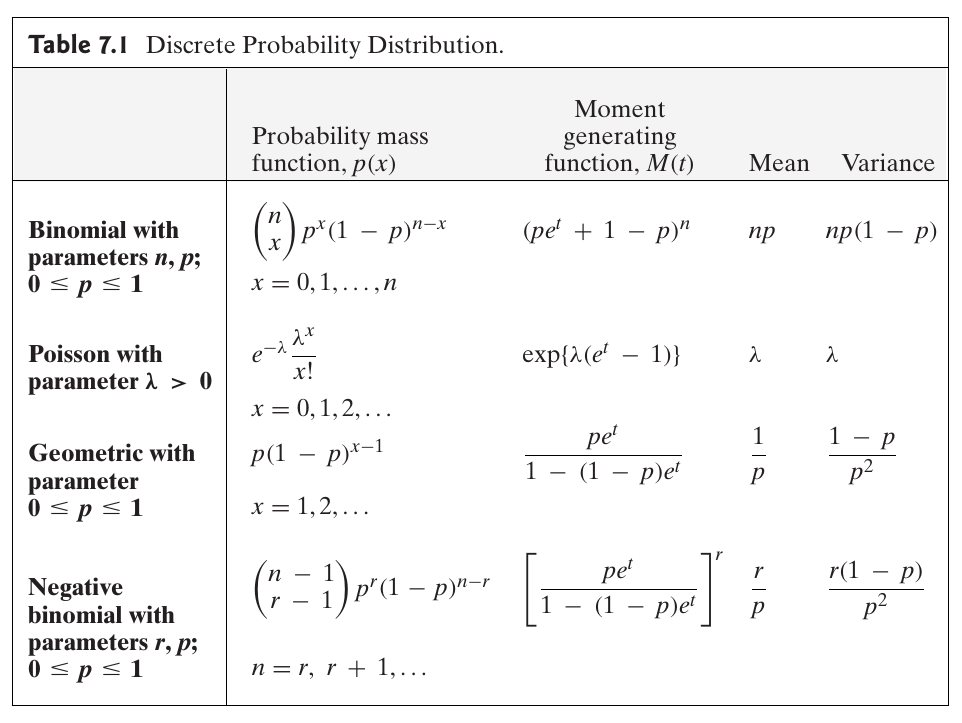
\includegraphics[scale=.5]{table1.PNG}
	\\
	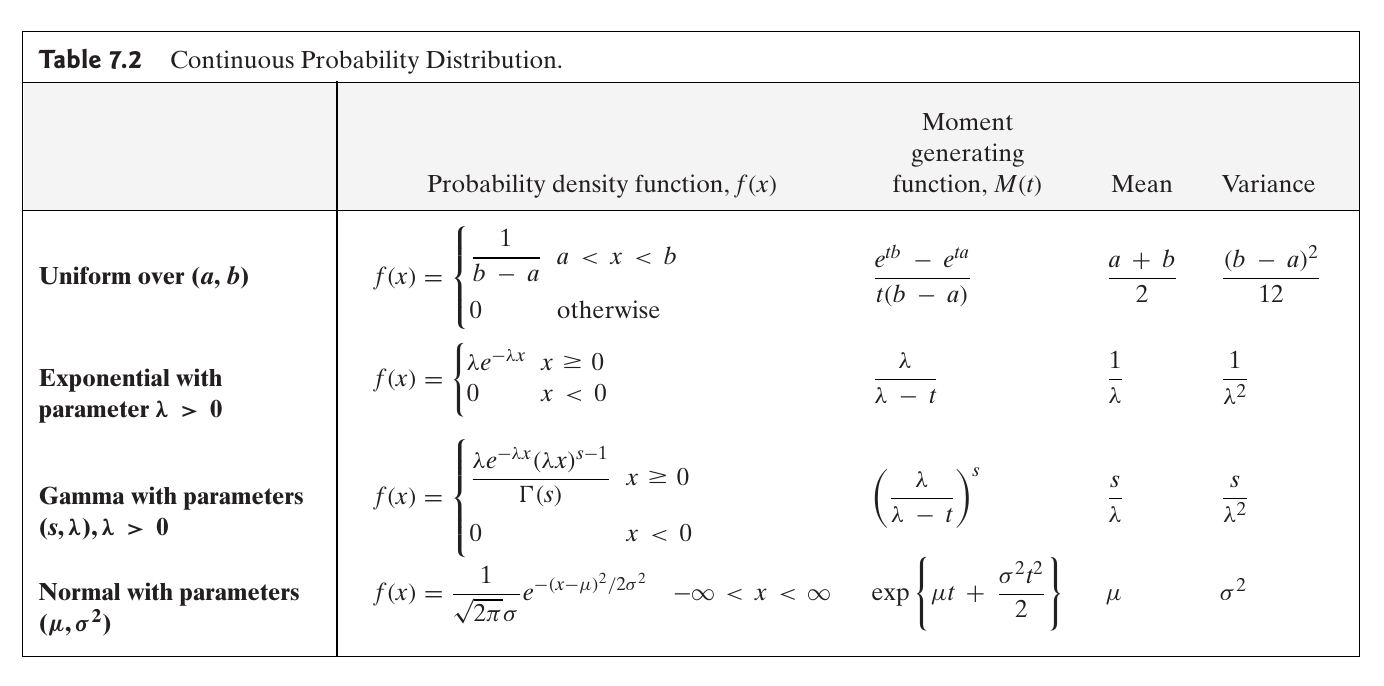
\includegraphics[scale=.5]{table2.PNG}
\end{centering}
\end{document}